\section{Triangle and Circle}

\begin{frame}{}
  \begin{center}
    {\bf Part II: Triangle and Circle}
  \end{center}
\end{frame}

\subsection{Angles}
\begin{frame}[fragile]{Angle between segments}

Given three points, $a$, $b$ and $o$, we can calculate
the angle between $\overline{oa}$ and $\overline{ob}$ using the dot product.\medskip

Given that: $oa\cdot ob = |oa|\times|ob|\times\cos(\theta)$, we have $\theta = \arccos(\frac{oa\cdot ob}{|oa|\times|ob|})$\bigskip

{\smaller

\begin{exampleblock}{}
\begin{verbatim}
#import <cmath>

// angle in radians (0..2*PI)
double angle(point a, point o, point b) {
  vec oa = toVector(o, a), ob = toVector(o, b);
  return acos(dot(oa, ob) / sqrt(norm_sq(oa) * norm_sq(ob)));
}
\end{verbatim}
\end{exampleblock}}
\end{frame}

\begin{frame}[fragile]{Left, Right and Collinear Points}

  Given a line defined by points $p$ and $q$, we are interested in knowing if point $r$ is on the left/right side of the line, or if the three ponts are collinear.\bigskip

  Let $\vec{pq}$ and $\vec{pr}$ be two vectors, the {\bf cross product} $\vec{pq} \times \vec{pr}$ is a vector that is perpendicular to both vectors. The  magnitude of the cross product is positive / zero / negative if $p \to q \to r$ is left turn / collinear / right turn.

  {\smaller
  \begin{exampleblock}{}
  \begin{verbatim}
  double cross(vec a, vec b) { return a.x * b.y - a.y * b.x; }

  bool ccw(point p, point q, point r) {
    return cross(toVec(p, q), toVec(p, r)) > 0; }

  collinear(point p, point q, point r) {
    return fabs(cross(toVec(p, q), toVec(p, r))) < EPS;
  \end{verbatim}
  \end{exampleblock}
  }
\end{frame}


\subsection{Circles}
\begin{frame}[fragile]
  \frametitle{Circles}
  \begin{itemize}
  \item A circle is stored as its center point $c$, and its radius $r$.\medskip

  \item The circle contains all points $(x,y)$ where $(x-a)^2+(y-b)^2 \leq r^2$\medskip

  \item No square root, so less chance of floating point errors.
  \end{itemize}\bigskip

  \begin{exampleblock}{Test if Point $p$ is inside Circle -- Integer Version}
    {\smaller
\begin{verbatim}
int insideCircle(point_i p, point_i c, int r) {
   int dx = p.x-c.x, dy = p.y-c.y;
   int Euc = dx*dx + dy*dy, rSq = r*r;
   return Euc < rSq ? 0 : Euc == rSq ? 1 : 2;
   // 0 - inside, 1 - border, 2- outside
}
\end{verbatim}
}
  \end{exampleblock}
\end{frame}


% \begin{frame}
%   \frametitle{Problem Example -- UVA 10589 Area}
%
%   \begin{columns}
%     \column{.4\textwidth}
%       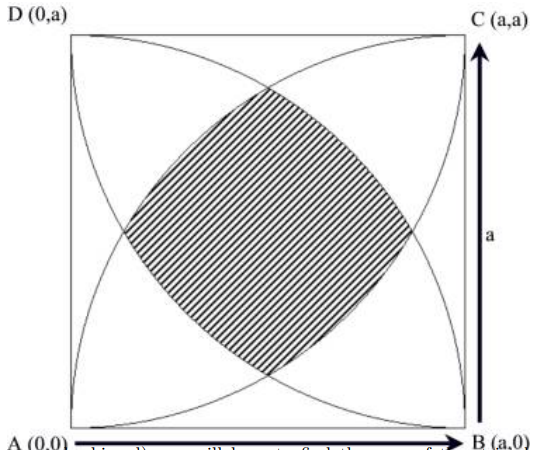
\includegraphics[width=1\textwidth]{img/area_uva}
%     \column{.6\textwidth}
%     {\bf QUIZ:}
%     \begin{itemize}
%       \item What is the area of the shaded part?
%       \item You know $a$, the radius of the 4 circles;
%     \end{itemize}\bigskip
%
%     \begin{block}{Monte Carlo Approach}
%       \begin{itemize}
%       \item Sample $N$ random points;
%       \item Calculate proportion $p$ of points in area;
%       \item Shaded area is $\frac{a^2}{p}$\bigskip
%
%       \item Mote Carlo approach is useful in several problems!
%       \end{itemize}
%     \end{block}
%   \end{columns}
% \end{frame}


% one dim measures: radius, diameter, circumference
% central angle, sector, arc
% chord: if you know the points, how to find the points if you know center and line
\begin{frame}
  \frametitle{Other circle properties}
    \begin{center}
      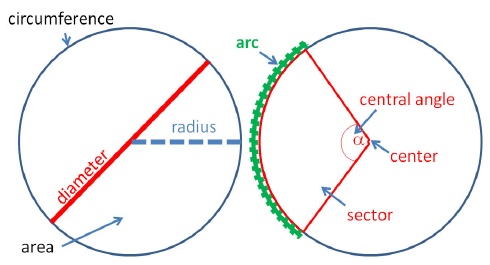
\includegraphics[width=0.5\textwidth]{../img/circle_halim0}
      \ppagenote{Circle Properties Images from Stephen Halim "Competitive Programming 3"}
    \end{center}

    \begin{itemize}
      \item {\bf radius:} $r$, {\bf diameter:} 2r, {\bf circumference:} $2\times\pi\times r$
      \item You can obtain $\pi$ from the problem, or with $\pi = 2\times \arccos(0)$
      \item Given a central angle $\alpha$:
      \begin{itemize}
        \item {\bf Arc:} $r\times\alpha$ (if in rad) or $r\times\frac{\alpha}{360}\times2\pi$ (if degrees)
        \item {\bf Sector:} $\frac{\alpha r^2}{2}$ (if in rad) or $2\pi r^2 \times \frac{\alpha}{360}$ (if degrees)
      \end{itemize}
    \end{itemize}
\end{frame}

\begin{frame}
  \frametitle{Other circle properties -- chord}
  \centering
    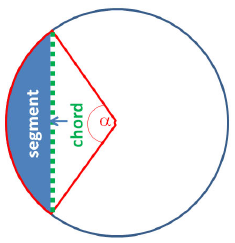
\includegraphics[width=0.25\textwidth]{../img/circle_halim1}

  \begin{itemize}
  \item {\bf chord:} Line segment with two ends in the circle's border.
  \item If you know $p_1$, $p_2$ and $c$, you can find $\alpha$ from the "angle" function;
  \item If you know $\alpha$ and $r$, you can find the size of the chord by: $|p_1p_2| = 2\times r\times\sin(\alpha/2)$
  \begin{itemize}
    \item {\bf Quiz:} If you know a line and a circle, how do you find $p_1$ and $p_2$?
  \end{itemize}
  \item If you know $p_1$, $p_2$, and $r$ (but not $\alpha$ or $c$), you can find the center of the circle using the code in the next page;
  \end{itemize}
\end{frame}

\begin{frame}[fragile]{Circle Center from points and radius}
  You have two points $p_1, p_2$ that form a chord in a circle, and the radius of that circle. How do you find the center?

  {\smaller
\begin{exampleblock}{}
\begin{verbatim}
bool circle2PtsRad(point p1, point p2, double r, point &c) {
  double d2 = (p1.x - p2.x) * (p1.x - p2.x) +
              (p1.y - p2.y) * (p1.y - p2.y);
  double det = r * r / d2 - 0.25;

  if (det < 0.0) return false; // Can't make circle

  double h = sqrt(det);
  c.x = (p1.x + p2.x) * 0.5 + (p1.y - p2.y) * h;
  c.y = (p1.y + p2.y) * 0.5 + (p2.x - p1.x) * h;
  return true;
}
// to get the other center, reverse p1 and p2
\end{verbatim}
\end{exampleblock}
  }
\end{frame}

\subsection{Triangles}

\begin{frame}
  \frametitle{Triangle Problem Example: Soya milk}
  \begin{block}{}
    \begin{itemize}
    \item {\bf Input}:\\
      The dimensions of a Milk box, and its inclination: $l, w, h, \theta$
    \item {\bf Output}:\\
      The amount of milk left in the box.
    \end{itemize}
  \end{block}

  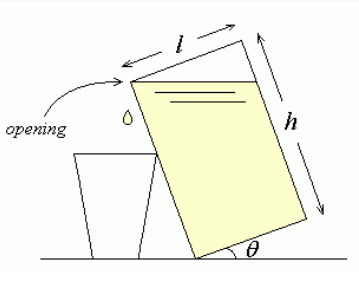
\includegraphics[width=0.4\textwidth]{img/milk_uva}
\end{frame}

\begin{frame}[t]
  \frametitle{Triangle/Circle Problem Example: Bounding Box}
  \begin{block}{}
    \begin{itemize}
      \item {\bf Input}: Three points that are the vertices of a {\bf regular polygon}, and number $n$ of sides in the polygon;\medskip
      \item {\bf Output}: Area of smallest {\bf axis aligned} rectangle that bounds this polygon.\medskip
    \end{itemize}
  \end{block}
\end{frame}

\begin{frame}
  \frametitle{Triangle Basic Facts}

    \begin{itemize}
    \item {\bf Triangle Inequality}: If $a,b,c$ are sides of a triangle, then $a+b > c; a+c > b; b+c > a$;\bigskip
    \item {\bf Perimeter, Semiperimeter}: $p = a+b+c$, $s = p/2$\bigskip
    \item {\bf Area}: $A = \frac{bh_b}{2}$\bigskip
    \item {\bf Area (Heron's formula)}: $A = \sqrt{s(s-a)(s-b)(s-c)}$\bigskip
    \item {\bf Triangulation}: Any 2D polygon can be decomposed into triangles;
  \end{itemize}
\end{frame}

\subsection{incircle}
\begin{frame}[fragile]{Incircle of a Triangle}
    \begin{columns}
      \column{0.15\textwidth}
      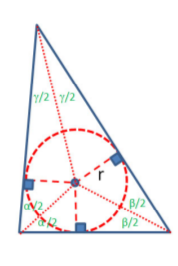
\includegraphics[width=1\textwidth]{../img/incircle_halim}
      \column{0.85\textwidth}
      \begin{itemize}
        \item An {\bf Inscribed Circle (incircle)} is the largest circle that fits inside a triangle;
        \item The radius of the incircle is: $r = A / s$
        \item The center of the circle can be found by the intersection of two {\bf angle bisectors}.
      \end{itemize}
      \end{columns}

    \begin{exampleblock}{Radius of the Incircle: $r = \text{area}/s$}
      {\smaller
\begin{verbatim}
double rInCircle(double ab, double bc, double ca) {
  return area(ab, bc, ca) / (0.5 * perimeter(ab, bc, ca)); }

double rInCircle(point a, point b, point c) {
  return rInCircle(dist(a, b), dist(b, c), dist(c, a)); }
\end{verbatim}}

    \end{exampleblock}
\end{frame}

\begin{frame}[fragile]
  \frametitle{Finding the center of the Incircle of a triangle}
  {\smaller
    \begin{exampleblock}{}
\begin{verbatim}
int inCircle(point p1, point p2, point p3, point &ctr, double &r) {
  r = rInCircle(p1, p2, p3);
  if (fabs(r) < EPS) return 0;            // Test colinear points !!!
  line l1, l2;    // we calculate the intersect of two angle bisectors

  double ratio; point p;
  ratio = dist(p1, p2) / dist(p1, p3);
  p = translate(p2, scale(toVec(p2, p3), ratio / (1 + ratio)));
  pointsToLine(p1, p, l1);                // bisector 1

  ratio = dist(p2, p1) / dist(p2, p3);
  p = translate(p1, scale(toVec(p1, p3), ratio / (1 + ratio)));
  pointsToLine(p2, p, l2);                // bisector 2

  areIntersect(l1, l2, ctr);              // find center (ctr)
  return 1;
}
\end{verbatim}
    \end{exampleblock}
    }
\end{frame}

\begin{frame}
  \frametitle{Circumcircle of a Triangle}
  \begin{columns}
    \column{0.3\textwidth}
    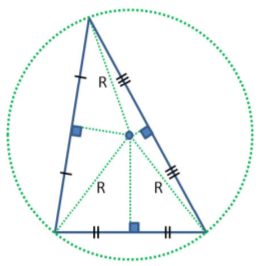
\includegraphics[width=1\textwidth]{../img/circumcircle_halim}
    \column{0.7\textwidth}
    \begin{itemize}
      \item The radius of the circumcircle in a triangle with sides $a,b,c$ and area A is $R = \frac{abc}{4A}$;
      \item The radius $R$ is also related to the {\bf Law of Sines}:
      \begin{equation*}
        \frac{a}{\sin{\alpha}} = \frac{b}{\sin{\beta}} = \frac{c}{\sin{\gamma}} = 2R
      \end{equation*}
    \end{itemize}
    \end{columns}\bigskip
    \begin{itemize}
      \item To find the center of the circumcircle:
      \begin{itemize}
        \item Use a similar algorithm as the center of the incirle (last slide);\medskip
        \item Instead of angle bisectors, use {\bf perpendicular bisectors};
      \end{itemize}
    \end{itemize}
\end{frame}
